\documentclass[../../../../main.tex]{subfiles}
\begin{document}

\begin{flushright}
\footnotesize\textit{【自動文字起こし・要確認】}
\end{flushright}

\begin{center}
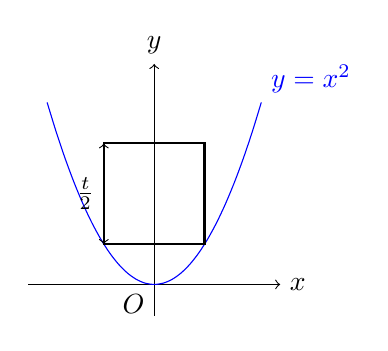
\begin{tikzpicture}[scale=0.8]
    % Parabola y = x^2
    \draw[->] (-2,0) -- (2,0) node[right] {$x$};
    \draw[->] (0,-0.5) -- (0,3.5) node[above] {$y$};
    \draw[domain=-1.7:1.7, smooth, variable=\x, blue] plot ({\x}, {\x*\x}) node[above right] {$y=x^2$};
    
    % Square 1
    \draw[thick] (-0.8, 0.64) -- (0.8, 0.64) -- (0.8, 2.24) -- (-0.8, 2.24) -- cycle;
    \draw[<->] (-0.8, 0.64) -- (-0.8, 2.24) node[midway, left] {$\frac{t}{2}$};
    \node[below left] at (0,0) {$O$};
\end{tikzpicture}
\qquad
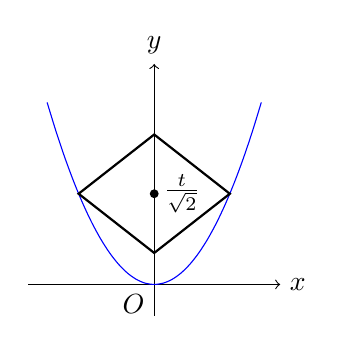
\begin{tikzpicture}[scale=0.8]
    % Parabola y = x^2
    \draw[->] (-2,0) -- (2,0) node[right] {$x$};
    \draw[->] (0,-0.5) -- (0,3.5) node[above] {$y$};
    \draw[domain=-1.7:1.7, smooth, variable=\x, blue] plot ({\x}, {\x*\x});
    
    % Diamond Square 2
    \draw[thick] (0, 0.5) -- (1.2, 1.44) -- (0, 2.38) -- (-1.2, 1.44) -- cycle;
    \fill (0,1.44) circle (2pt) node[right] {$\frac{t}{\sqrt{2}}$};
    \node[below left] at (0,0) {$O$};
\end{tikzpicture}
\qquad
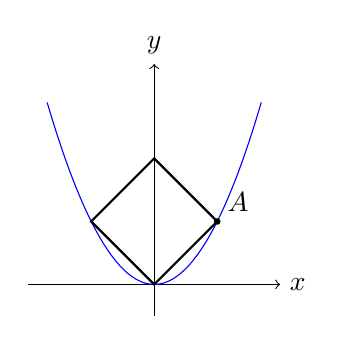
\begin{tikzpicture}[scale=0.8]
    % Parabola y = x^2
    \draw[->] (-2,0) -- (2,0) node[right] {$x$};
    \draw[->] (0,-0.5) -- (0,3.5) node[above] {$y$};
    \draw[domain=-1.7:1.7, smooth, variable=\x, blue] plot ({\x}, {\x*\x});
    
    % Diamond Square 3 at Origin
    \draw[thick] (0,0) -- (1, 1) node[above right] {$A$} -- (0, 2) -- (-1, 1) -- cycle;
    \fill (1,1) circle (1.5pt);
\end{tikzpicture}
\end{center}

[解] 中心が $y$ 軸上にないものは、中心が $y$ 軸上にくるよう平行移動することで、より $y$ 座標を小さくできるから、中心が $y$ 軸上にあるもののみ考える。この時、$y$ 座標が最小になるのは、以下のいずれか

\begin{enumerate}
  \item[$1^\circ$] 正方形の下2辺が $y=x^2$ にある
  \item[$2^\circ$] 正方形の対角線上の点2つが $y=x^2$ にある
  \item[$3^\circ$] 1つの頂点が原点にある
\end{enumerate}

以下、$y$ 座標 $f(t)$ とおく。($t > 0$)

$1^\circ$ の時
\[
f_1(t) = \left(\frac{t}{2}\right)^2 + \frac{t}{2} = \frac{1}{4}t^2 + \frac{1}{2}t
\]

$2^\circ$ の時
\[
f_2(t) = \left(\frac{t}{\sqrt{2}}\right)^2
\]
であり、この時、一番下の頂点 $(0, f(t) - \frac{t}{\sqrt{2}})$ が原点より上にあることが必要で、
\[
f(t) - \frac{t}{\sqrt{2}} = \frac{t}{2}\cdot t - \frac{t}{\sqrt{2}} = \frac{t}{\sqrt{2}}\left(\frac{t}{\sqrt{2}} - 1\right) \geqq 0 \iff t \geqq \sqrt{2} \quad (\because t > 0)
\]

$3^\circ$ の時、
\[
f_3(t) = \frac{t}{\sqrt{2}}
\]
であり、この時、$3^\circ$ の図の $A$ が $y=x^2$ に含まれていることが必要で、
\[
\frac{t}{\sqrt{2}} \geqq \left(\frac{t}{\sqrt{2}}\right)^2 \iff 0 < t \leqq \sqrt{2}
\]

以上のうち、$\min$ のものがもとめる関数である。これらを図示して右上図を得る

\begin{center}
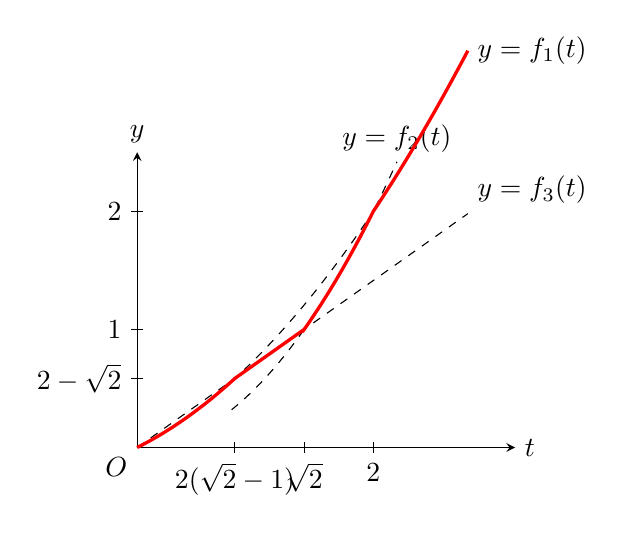
\begin{tikzpicture}[scale=1.5, >=stealth]
    \draw[->] (0,0) -- (3.2,0) node[right] {$t$};
    \draw[->] (0,0) -- (0,2.5) node[above] {$y$};
    \node[below left] at (0,0) {$O$};

    % Points on t-axis
    \draw (0.828, 0.05) -- (0.828, -0.05) node[below] {$2(\sqrt{2}-1)$};
    \draw (1.414, 0.05) -- (1.414, -0.05) node[below] {$\sqrt{2}$};
    \draw (2.0, 0.05) -- (2.0, -0.05) node[below] {$2$};

    % Values on y-axis
    \draw (0.05, 0.586) -- (-0.05, 0.586) node[left] {$2-\sqrt{2}$};
    \draw (0.05, 1.0) -- (-0.05, 1.0) node[left] {$1$};
    \draw (0.05, 2.0) -- (-0.05, 2.0) node[left] {$2$};

    % Curves
    \draw[dashed, domain=0:2.8, smooth, variable=\t] plot ({\t}, {0.25*\t*\t + 0.5*\t}) node[right] {$y=f_1(t)$};
    \draw[dashed, domain=0:2.8, smooth, variable=\t] plot ({\t}, {\t/1.414}) node[above right] {$y=f_3(t)$};
    \draw[dashed, domain=0.8:2.2, smooth, variable=\t] plot ({\t}, {0.5*\t*\t}) node[above] {$y=f_2(t)$};

    % Thick lower envelope f(t)
    \draw[very thick, red] (0,0) 
        -- plot[domain=0:0.828, smooth, variable=\t] ({\t}, {0.25*\t*\t + 0.5*\t})
        -- plot[domain=0.828:1.414, smooth, variable=\t] ({\t}, {\t/1.414})
        -- plot[domain=1.414:2.0, smooth, variable=\t] ({\t}, {0.5*\t*\t})
        -- plot[domain=2.0:2.8, smooth, variable=\t] ({\t}, {0.25*\t*\t + 0.5*\t});
\end{tikzpicture}
\end{center}

よって求める関数は
\[
f(t) = \begin{cases}
\frac{t}{\sqrt{2}} & (2(\sqrt{2}-1) \leqq t \leqq \sqrt{2}) \\
\frac{1}{2} t^2 & (\sqrt{2} \leqq t \leqq 2) \\
\frac{1}{4} t^2 + \frac{1}{2} t & (0 < t \leqq 2(\sqrt{2}-1), \ 2 \leqq t)
\end{cases}
\quad \text{/\!\!/}
\]
である

\end{document}
